% Generated from figures/generated/ch09-transaction.svg; do not hand edit.
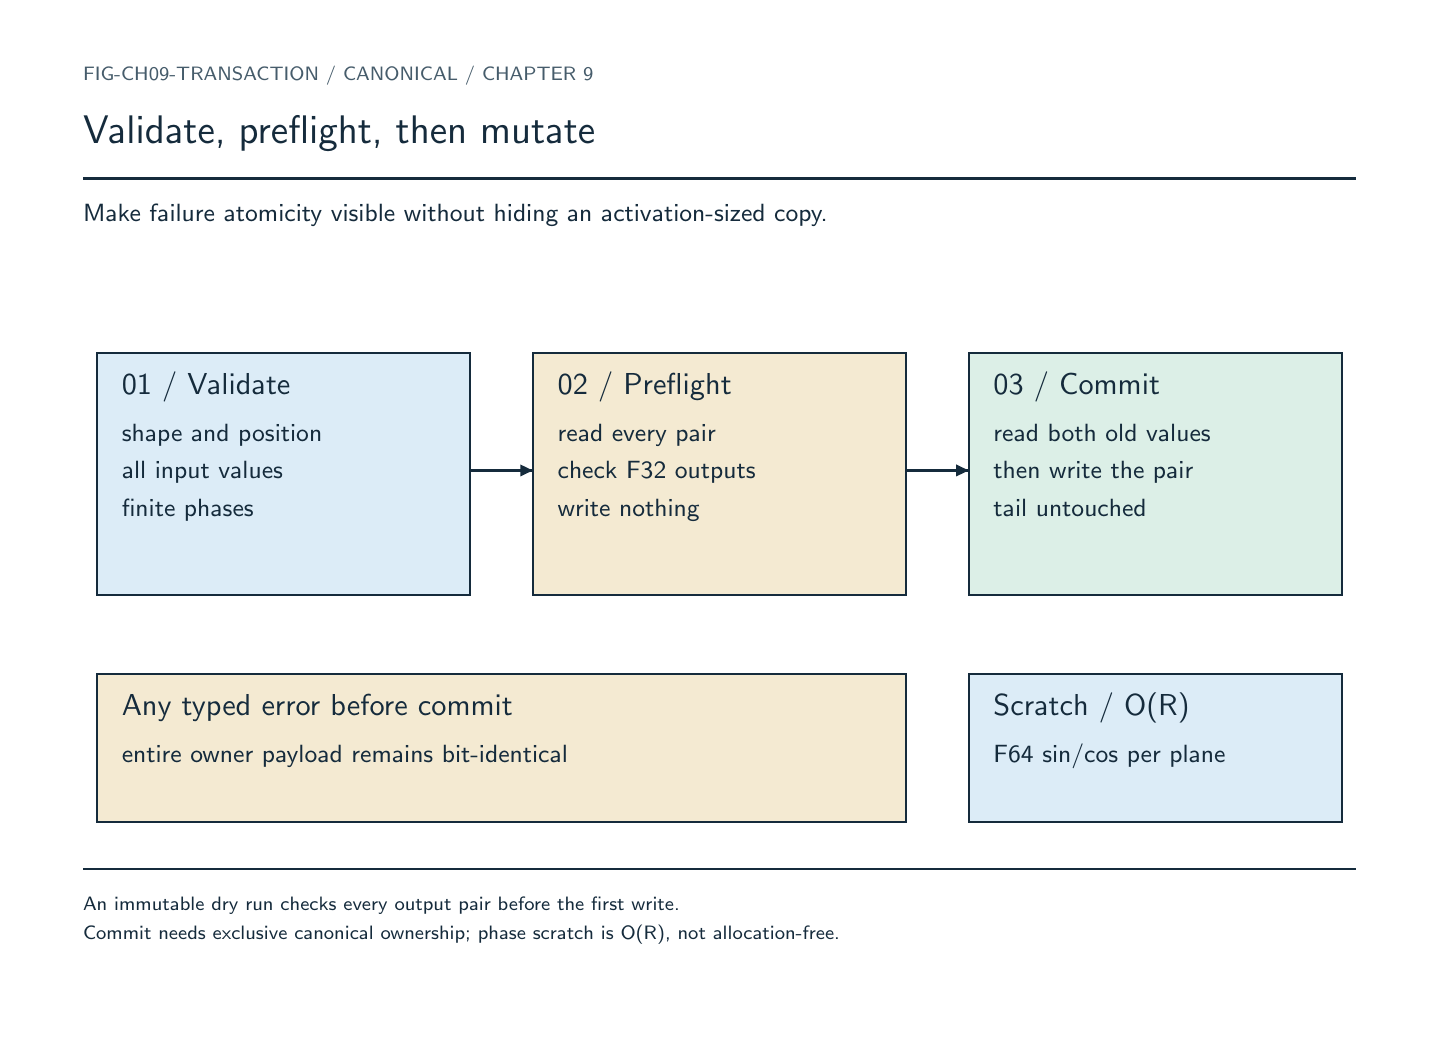
\begin{tikzpicture}[x=.5pt,y=-.5pt]
\path[use as bounding box] (0,0) rectangle (1000,720);
\path[fill=white,draw=none,line width=0.5pt] (0.0,0.0) rectangle (1000.0,720.0);
\node[inner sep=0pt,outer sep=0pt,anchor=base west,text={rgb,255:red,70;green,92;blue,107},font=\sffamily\fontsize{7.0}{8.4}\selectfont] at (40,38) {FIG-CH09-TRANSACTION  /  CANONICAL / CHAPTER 9};
\node[inner sep=0pt,outer sep=0pt,anchor=base west,text={rgb,255:red,21;green,43;blue,60},font=\sffamily\fontsize{15.0}{18.0}\selectfont] at (40,84) {Validate, preflight, then mutate};
\draw[fill=none,draw={rgb,255:red,21;green,43;blue,60},line width=0.75pt] (40,109) -- (960,109);
\node[inner sep=0pt,outer sep=0pt,anchor=base west,text={rgb,255:red,21;green,43;blue,60},font=\sffamily\fontsize{9.5}{11.4}\selectfont] at (40,140) {Make failure atomicity visible without hiding an activation-sized copy.};
\path[fill={rgb,255:red,220;green,236;blue,247},draw={rgb,255:red,21;green,43;blue,60},line width=0.7pt] (50.0,235.0) rectangle (320.0,410.0);
\node[inner sep=0pt,outer sep=0pt,anchor=base west,text={rgb,255:red,21;green,43;blue,60},font=\sffamily\fontsize{9.5}{11.4}\selectfont] at (64,264) {};
\node[inner sep=0pt,outer sep=0pt,anchor=base west,text={rgb,255:red,21;green,43;blue,60},font=\sffamily\fontsize{10.5}{12.6}\selectfont] at (68,265) {01 / Validate};
\node[inner sep=0pt,outer sep=0pt,anchor=base west,text={rgb,255:red,21;green,43;blue,60},font=\sffamily\fontsize{9.0}{10.799999999999999}\selectfont] at (68,299) {shape and position};
\node[inner sep=0pt,outer sep=0pt,anchor=base west,text={rgb,255:red,21;green,43;blue,60},font=\sffamily\fontsize{9.0}{10.799999999999999}\selectfont] at (68,326) {all input values};
\node[inner sep=0pt,outer sep=0pt,anchor=base west,text={rgb,255:red,21;green,43;blue,60},font=\sffamily\fontsize{9.0}{10.799999999999999}\selectfont] at (68,353) {finite phases};
\path[fill={rgb,255:red,244;green,234;blue,210},draw={rgb,255:red,21;green,43;blue,60},line width=0.7pt] (365.0,235.0) rectangle (635.0,410.0);
\node[inner sep=0pt,outer sep=0pt,anchor=base west,text={rgb,255:red,21;green,43;blue,60},font=\sffamily\fontsize{9.5}{11.4}\selectfont] at (379,264) {};
\node[inner sep=0pt,outer sep=0pt,anchor=base west,text={rgb,255:red,21;green,43;blue,60},font=\sffamily\fontsize{10.5}{12.6}\selectfont] at (383,265) {02 / Preflight};
\node[inner sep=0pt,outer sep=0pt,anchor=base west,text={rgb,255:red,21;green,43;blue,60},font=\sffamily\fontsize{9.0}{10.799999999999999}\selectfont] at (383,299) {read every pair};
\node[inner sep=0pt,outer sep=0pt,anchor=base west,text={rgb,255:red,21;green,43;blue,60},font=\sffamily\fontsize{9.0}{10.799999999999999}\selectfont] at (383,326) {check F32 outputs};
\node[inner sep=0pt,outer sep=0pt,anchor=base west,text={rgb,255:red,21;green,43;blue,60},font=\sffamily\fontsize{9.0}{10.799999999999999}\selectfont] at (383,353) {write nothing};
\path[fill={rgb,255:red,220;green,239;blue,231},draw={rgb,255:red,21;green,43;blue,60},line width=0.7pt] (680.0,235.0) rectangle (950.0,410.0);
\node[inner sep=0pt,outer sep=0pt,anchor=base west,text={rgb,255:red,21;green,43;blue,60},font=\sffamily\fontsize{9.5}{11.4}\selectfont] at (694,264) {};
\node[inner sep=0pt,outer sep=0pt,anchor=base west,text={rgb,255:red,21;green,43;blue,60},font=\sffamily\fontsize{10.5}{12.6}\selectfont] at (698,265) {03 / Commit};
\node[inner sep=0pt,outer sep=0pt,anchor=base west,text={rgb,255:red,21;green,43;blue,60},font=\sffamily\fontsize{9.0}{10.799999999999999}\selectfont] at (698,299) {read both old values};
\node[inner sep=0pt,outer sep=0pt,anchor=base west,text={rgb,255:red,21;green,43;blue,60},font=\sffamily\fontsize{9.0}{10.799999999999999}\selectfont] at (698,326) {then write the pair};
\node[inner sep=0pt,outer sep=0pt,anchor=base west,text={rgb,255:red,21;green,43;blue,60},font=\sffamily\fontsize{9.0}{10.799999999999999}\selectfont] at (698,353) {tail untouched};
\draw[fill=none,draw={rgb,255:red,21;green,43;blue,60},line width=1.25pt] (320,320) -- (365,320);
\path[fill={rgb,255:red,21;green,43;blue,60},draw=none,line width=0.5pt] (365.00,320.00) -- (356.00,324.35) -- (356.00,315.65) -- cycle;
\draw[fill=none,draw={rgb,255:red,21;green,43;blue,60},line width=1.25pt] (635,320) -- (680,320);
\path[fill={rgb,255:red,21;green,43;blue,60},draw=none,line width=0.5pt] (680.00,320.00) -- (671.00,324.35) -- (671.00,315.65) -- cycle;
\path[fill={rgb,255:red,244;green,234;blue,210},draw={rgb,255:red,21;green,43;blue,60},line width=0.7pt] (50.0,467.0) rectangle (635.0,574.0);
\node[inner sep=0pt,outer sep=0pt,anchor=base west,text={rgb,255:red,21;green,43;blue,60},font=\sffamily\fontsize{9.5}{11.4}\selectfont] at (64,496) {};
\node[inner sep=0pt,outer sep=0pt,anchor=base west,text={rgb,255:red,21;green,43;blue,60},font=\sffamily\fontsize{10.5}{12.6}\selectfont] at (68,497) {Any typed error before commit};
\node[inner sep=0pt,outer sep=0pt,anchor=base west,text={rgb,255:red,21;green,43;blue,60},font=\sffamily\fontsize{9.0}{10.799999999999999}\selectfont] at (68,531) {entire owner payload remains bit-identical};
\path[fill={rgb,255:red,220;green,236;blue,247},draw={rgb,255:red,21;green,43;blue,60},line width=0.7pt] (680.0,467.0) rectangle (950.0,574.0);
\node[inner sep=0pt,outer sep=0pt,anchor=base west,text={rgb,255:red,21;green,43;blue,60},font=\sffamily\fontsize{9.5}{11.4}\selectfont] at (694,496) {};
\node[inner sep=0pt,outer sep=0pt,anchor=base west,text={rgb,255:red,21;green,43;blue,60},font=\sffamily\fontsize{10.5}{12.6}\selectfont] at (698,497) {Scratch / O(R)};
\node[inner sep=0pt,outer sep=0pt,anchor=base west,text={rgb,255:red,21;green,43;blue,60},font=\sffamily\fontsize{9.0}{10.799999999999999}\selectfont] at (698,531) {F64 sin/cos per plane};
\draw[fill=none,draw={rgb,255:red,21;green,43;blue,60},line width=0.75pt] (40,608) -- (960,608);
\node[inner sep=0pt,outer sep=0pt,anchor=base west,text={rgb,255:red,21;green,43;blue,60},font=\sffamily\fontsize{7.5}{9.0}\selectfont] at (40,638) {An immutable dry run checks every output pair before the first write.};
\node[inner sep=0pt,outer sep=0pt,anchor=base west,text={rgb,255:red,21;green,43;blue,60},font=\sffamily\fontsize{7.5}{9.0}\selectfont] at (40,659) {Commit needs exclusive canonical ownership; phase scratch is O(R), not allocation-free.};
\end{tikzpicture}
